\documentclass{ieeeaccess}
\usepackage{cite}
\usepackage{amsmath,amssymb,amsfonts}
\usepackage{graphicx}
\usepackage{textcomp}
\usepackage{multirow}
\usepackage{mathtools}
\usepackage{subfigure}
\DeclarePairedDelimiter{\abs}{\lvert}{\rvert}
\def\BibTeX{{\rm B\kern-.05em{\sc i\kern-.025em b}\kern-.08em
T\kern-.1667em\lower.7ex\hbox{e}\kern-.125emX}}

\usepackage{algorithm}
\usepackage{colortbl}
\usepackage{algpseudocode}
\usepackage{tabularx}
\usepackage{arydshln}
% \usepackage[algcompatible]{algpseudocode}
\usepackage{array}
\newlength\savedwidth
\newcommand{\wcline}[1]{\noalign{\global\savedwidth\arrayrulewidth\global\arrayrulewidth 1.0pt} \cline{#1}
\noalign{\global\arrayrulewidth\savedwidth}}

\newcommand{\CCI}{\mathrm{CCI}} 
\newcommand{\HFDI}[1]{H_{image}(#1)}
\newcommand{\ti}{an evasion-resilient IoT malware detection scheme with invalidating adversarial byte sequences and 1D convolutional filters}
\newcommand{\TI}{An Evasion-Resilient IoT Malware Detection Scheme with Invalidating Adversarial Byte Sequences and 1D Convolutional Filters}

\newcommand{\myfigurename}{Fig.}
\newcommand{\mytablename}{Table}
% Require$B$H(BEnsure$B$r(BInput$B$H(BOutput$B$K$9$k(B
\renewcommand{\algorithmicrequire}{\textbf{Input:}}
\renewcommand{\algorithmicensure}{\textbf{Output:}}
\newcommand{\etal}{\textit{et~al.}}


\begin{document}
\history{Date of publication xxxx 00, 0000, date of current version xxxx 00, 0000.}
\doi{10.1109/ACCESS.2017.DOI}

\title{An Evasion-Resilient IoT Malware Detection Scheme with Invalidating Adversarial Byte Sequences and 1D Convolutional Filters} 

\author{
  \uppercase{Kosuke Igarashi}\authorrefmark{1},
  \uppercase{Hiroya Kato}\authorrefmark{1}, \IEEEmembership{Graduate Student Member, IEEE},
  and \uppercase{Iwao Sasase}.\authorrefmark{1}, \IEEEmembership{Senior Member, IEEE}}
\address[1]{Department of Information and Computer Science, Faculty of Science and Technology, Keio University 3-14-1 Hiyoshi, Kohoku, Yokohama, Kanagawa 223-8522, Japan}
% \tfootnote{This work is partly supported by the Grant in Aid for Scientific Research (No.17K06440) from Japan Society for Promotion of Science (JSPS).}

\markboth
{Igarashi \headeretal: \TI}
{Igarashi \headeretal: \TI}

\corresp{Corresponding author: Kosuke Igarashi (e-mail: igarashi@sasase.ics.keio.ac.jp).}

\begingroup
\newlength{\xfigwd}
\setlength{\xfigwd}{\textwidth}

\begin{abstract}
Detecting Internet of Things (IoT) malware robustly against evasive techniques is imperative.
As an IoT malware detection scheme, we focus on the scheme leveraging binary-derived grayscale images for Convolutional Neural Network (CNN) in IoT device detection because it can cope with the accelerating IoT malware surge due to the automatic and light-weight analysis which CNN can realize.
However, that scheme can be evaded by the adversary with manipulated malware grayscale image or binary data.
In this thesis, we propose an evasion-resilient IoT malware detection scheme with invalidating adversarial byte sequences and 1D convolutional filters.
The valuable regions still remain which contribute to classification in both manipulated targets, grayscale image and binary data, after the attacks.
Thus, I improve the detection accuracy by statically extracting/enhancing valuable region of each manipulated target to the CNN model.
By evaluation with each manipulated dataset, we show our scheme can improve detection performance against both evasive techniques. 
Exploring the valuable regions remaining in manipulated target and improvement of the detection accuracy utilizing the regions in my detection are the contributions of my research. 
\end{abstract}

\begin{keywords} 
 IoT malware detection, Convolutional Neural Network, Obfuscation, Adversarial Examples 
 \end{keywords}

\titlepgskip=-15pt

\maketitle

\section{Introduction}  \label{sec:introduction}
In these days, the Internet of Things (IoT) is interconnetcting a large number of electronic devices with a variety of applications in our lives, such as smart appliances, smart houses, smart grid, energy management systems, and so on, at a tremendous speed.
The number of the IoT devices is continuously increased.
It is estimated to be about 50 billion all over the world by 2030 \cite{bg1, bg2}.
They become targets of malware attacks due to the rapid increase and the development into devices which have interconnectivity in these days.
Unfortunately, vulnerable IoT devices are spreading since the countermeasures cannot keep up with this trend of IoT malware attacks.
\figurename~\ref{fig:mirai} represents an actual case of attack damage by malware called Mirai.
In fact, as shown in \figurename~\ref{fig:mirai}, attacks against companies using many IoT devices infected with malware have become a problem, and the detection of IoT malware has become an urgent issue.
Thus, this circumstance results in the urgency of detecting IoT malware.

\begin{figure}[t]
 \centering
 %\hspace{-55pt}
 \includegraphics[scale=0.28]{./figures/mirai.pdf}
 \caption{The case of attack damage by Mirai malware.} 
 \label{fig:mirai}
\end{figure}
%\afterpage{\clearpage}
%\newpage
Existing solutions for detecting malware are mainly classified into router-side schemes \cite{net} and device-side schemes \cite{om, hwang, cfg, cfg2}.

Router-side schemes pay attention to the fact that there exist strong evidences of malware in network traffic.
This is because adversaries have to scan IoT devices and propagate their malware before attacking itself and these phases cause abnormal traffic which cannot be seen in benign case.
Based on the fact, those scheme utilize the features extracted from incoming packets in the scanning/propagation phase such as destination IP address during a certain time, port number and so on, at a gateway of the network.
Although router-side schemes are useful, these schemes are subject to internal attacks of the local network itself since the packets do not go through the router.

In order to cope with the limitations of router-side schemes, device-side schemes are proposed.
Device-side schemes are conducted by utilizing the features extracted from malware itself at each IoT devices.
Most of the device-side schemes utilze various features which can be extracted statically since IoT devices are not suitable for dynamic detections due to their limited computing and storage capabilities.
Kumar et al. utilezes the features regarding to Control Flow Graphs (CFGs) acquired by complicated analysis and definitions of the features \cite{cfg}.
Although that scheme can extract represantative features of the application, it is a time-consuming and laborious method due to the analysis for an enormous number of IoT malware.

In order to cope with the spreading IoT malware with device-side detections, some researchers utilize Convolutional Neural Network (CNN) in their scheme.
Su et al. utilezes GrayScale Image (GSI) converted from raw bytes of each malware binary for its CNN \cite{previous}.
Although it is suitable for IoT malware detection since CNN can extract malware features from GSI automatically without feature engineering, it can be avoided with evasive techniques by adversaries to GSI or Binary Data (BD) of malware. 

In order to detect such malware with exisiting evasive techniques, that is manipulated GSIs and BD, in this thesis, we propose an evasion-resilient IoT malware detection scheme with invalidating adversarial byte sequences and 1D convolutional filters.
The main idea of our scheme is that the some regions which contribute to decision making in each manipulated target still remain after the evasive techniques by adverasaries. 
This research aims to improve the detection accuracy by statically by statically extracting/enhancing each beneficial region of the manipulated target for the CNN model.

The contributions of this thesis are as follows: 
\begin{itemize}
 \item I find the valuable regions which remain in adversarial malware and improve the detection accuracy of them by denoising procedure.
 \item I find the valuable features which obfuscated malware have and improve the detection accuracy of them by emphasizeing their valuable regions to CNN model.
 \item To the best of my knowledge, there is currenlty no reference to research defense schemes against the evasive techniques by adversaries. However, it is considered in this thesis, and, furthermore, give effective solutions.
\end{itemize}

The rest of this thesis is constructed as follows. 
After this introduction, related work are introduced in Section \ref{sec:related_work}.
The previous scheme and the issues of that scheme are explained in Section \ref{sec:previous_scheme}.
Proposed scheme is described in Section \ref{sec:proposed_scheme}.
Various evaluation results are shown in Section \ref{sec:evaluation}.
Finally, the conclusions of this thesis are presented in Section \ref{sec:conclusion}.


\section{Related Work} \label{sec:related_work}
In order to detect IoT malware, several schemes have been proposed. 
These schemes are divided into router-side detection and device-side detection.
Router-side detection is performed at a gateway on the basis of the features regarding propagation behavior for building a botnet.
Meanwhile, device-side detection is conducted at each IoT device by utilizing static features extracted from malware itself.
The representative schemes are explained in the following subsections.

\subsection{Router-side detection}
Router-side detctions leverage the fact that there exists strong evidence of malware in network traffic.
Kumar et al. \cite{net} propose the scheme focusing on network traffic while the scanning and propagation phase in particular which is observed in most of the existing malware behaviour for the purpose of building a botnet as shown in \figurename~\ref{fig:lan}.
Bots scanning for and infecting vulnerable devices are targeted in particular that scheme. 
This is because the scanning and propagation phase of the botnet life-cycle stretches over many months and that scheme can detect and isolate the bots before they can participate in an actual attack such as DDoS.
Based on the fact above, that scheme detects abnormal traffic caused while this phase which cannot be seen in benign cases utilizing machine learning.
It utilizes the number of unique destination IP addresses and packets per destination IP addresses as features observing incoming packets which have spcific target destination port number that the existing malware tend to send.
The number of unique destination IP addresses in case of malware-induced scanning traffic will be far more than benign traffic since the malware generates random IP addresses and sends malicious requests to them.
Also, the number of packets per destination IP addresses seeks to exploit the fact that malware typically does not send mulitiple malicious packets to the same IP addresses (only a single packet is sent in most cases), possibly to cover as many devices as possible during the scanning/propagation phase.

By being based on the scanning/propagation phase, it can detect and isolate the bots before they can participate in an actual attack such as DDoS.

However, that scheme is subject to local network attacks where IoT devices are targeted directly by adversaries in the same local network.
Thus, exploring the malware detection schemes which can be realized by each IoT device is needed due to the vulnerability against local network attacks.

\begin{figure}[h]
 \centering
 %\hspace{-55pt}
 \includegraphics[scale=0.28]{./figures/lan.pdf}
 \caption{The router-side detection in the scanning/propagation flow and its problem.} 
 \label{fig:lan}
\end{figure}
%\afterpage{\clearpage}
%\newpage

\subsection{Device-side detection} 
Device-side detection schemes are conducted by utilizing the features extracted from malware file itself at each device on the basis of malware, and they tend to have similality since adversaries make them based on the existing ones \cite{om, hwang, cfg, cfg2}.
Most of them utilize various features which can be extracted statically since IoT devices are not suitable for dynamic approach due to their limited computing and storage capabilities.

Torabi et al. propose the scheme which utilizes meaningful strings from the binary code, such as IP addresses of adversarial hosts (e.g., C\&C servers) and/or embedded commands/payloads \cite{om}.
That scheme focus on the fact that IoT malware need to communicate with adversarial hosts to obtain malicious command/payload and upload gathered information.
This is typically achieved by embedding a series of commands and IP addresses to ensure successful post-infection communication for operating further malicious activities. 
Although that scheme realizes lightweight static detection with simple reverse-engineering techniques, its detection can be easily avoided by malware where the meaningful strings are obfuscated in order to hide them with simple obfuscation techniques.
Such obfuscation techniques can be applied even on IoT devices where the computing and storage capabilities are limited.

Hwang et al. also use string information from binary data \cite{hwang}.
They extract around 1800 different strings including API names, DLL names, library function names of programming languages and PE/ELF file formats.
The major limitation of their work is also that their method may not be effective over packed or encrypted samples because their method depends only on the strings available explicitly, and such packed/encrypted samples reveal limited string information during static analysis.

In order to avoid easily detection rejection by adversaries, researchers propose the scheme which utilizes the features acquired from a Control Flow Graph (CFG), which could be used to extract representative static features of the application as shown in \figurename~\ref{fig:cfg} \cite{cfg, cfg2}.
The theoretic metrics of CFGs, such as the number of edges, density of a graph, shortest paths between each node and so on, can be multiple features of the model effctively derived from malware constructions under the limitation of static approach.
Alasmary et al. focus on the fact that some defferences in those metrics can be observed between benign software and IoT malware \cite{cfg}.
In that research, they reveal that IoT malware, and also each malware family, have various algorithmic and structural properties through complex analysis of CFGs acquired from about 6000 malware and benign software as shown in \figurename~\ref{fig:cfg}. 
Utilizing such properties of the CFGs, that scheme realize high accurate detection.
However, that scheme is a time-consuming and laborious method due to the feature engineering for exploring effective metrics with analysing an enormous number of IoT malware.

\begin{figure}[h]
 \centering
 %\hspace{-55pt}
 \includegraphics[scale=0.28]{./figures/cfg.pdf}
 \caption{The overview of device-side detection using CFG.} 
 \label{fig:cfg}
\end{figure}

\section{Previous scheme} \label{sec:previous_scheme}
\subsection{Overview} 
In order to deal with spreading IoT malware with device-side detections in more practical means, CNN is utilized in the previous scheme \cite{previous}.
Our research is more practical scheme which applys this device-side detection with CNN improving its issues.
The main idea of the previous scheme is that there exists the difference of GSIs converted from each malware Binary Data (BD) which is always acquired in IoT devices due to the exectable format of them.
In that scheme \cite{previous}, a malware binary is reformatted as an 8-bit sequence and then be converted to a GSI which has one channel and pixel values from 0 to 255.
To confirm the performance of the scheme, some samples of malware and benign software GSIs are prepared in our research and shown by \figurename~\ref{fig:malGSI} and \figurename~\ref{fig:benGSI}.
By comparison, some novel differences between them can be observed even by human eyes.
For example, it can be seen that malware GSIs always are more dense.
On the other hand, the GSI of benign softwares tends to have larger header parts than malware.

These GSIs can represents each features and be fed into CNN.
Since, CNN can extract effective features from these GSI automatically by learning deep non-linear features even that can be hardly descovered and understood by human eyes.
Furthermore, once trained, the network itself is lightweight and can be run with tiny computational resources, since only the trained parameters and information of network structure are kept.
Thus, CNN is a suitable scheme for IoT malware detections since it does not demand feature engineering and also computational costs while the detection.

\begin{figure}[h]
 \centering
 %\hspace{-55pt}
 \includegraphics[scale=0.28]{./figures/malGSI.pdf}
 \caption{The malware GSIs.} 
 \label{fig:malGSI}
\end{figure}
%\afterpage{\clearpage}
%\newpage
\begin{figure}[h]
 \centering
 %\hspace{-55pt}
 \includegraphics[scale=0.28]{./figures/benGSI.pdf}
 \caption{The benign file GSIs.} 
 \label{fig:benGSI}
\end{figure}
%\afterpage{\clearpage}

\subsection{Issues} 
Although the previous scheme can cope with spreading IoT malware with device-side detection in more practical means, it is susceptible to evasive techniques against the inputs of the CNN, GSIs and binary \cite{attack1, attack2}.
Adversaries can evade the CNN based detection with two evasive techniques against each input as shown in \figurename~\ref{fig:ov}.
Malwares whose GSIs are manipulated to evade the detection are called Adversarial Malware (AM) and also malware whose binary is manipulated are called Obfuscated Malware (OM) in this research.  
The representative vulnerabilities against each attack are explained in the following subsections.

\begin{figure}[h]
 \centering
 %\hspace{-55pt}
 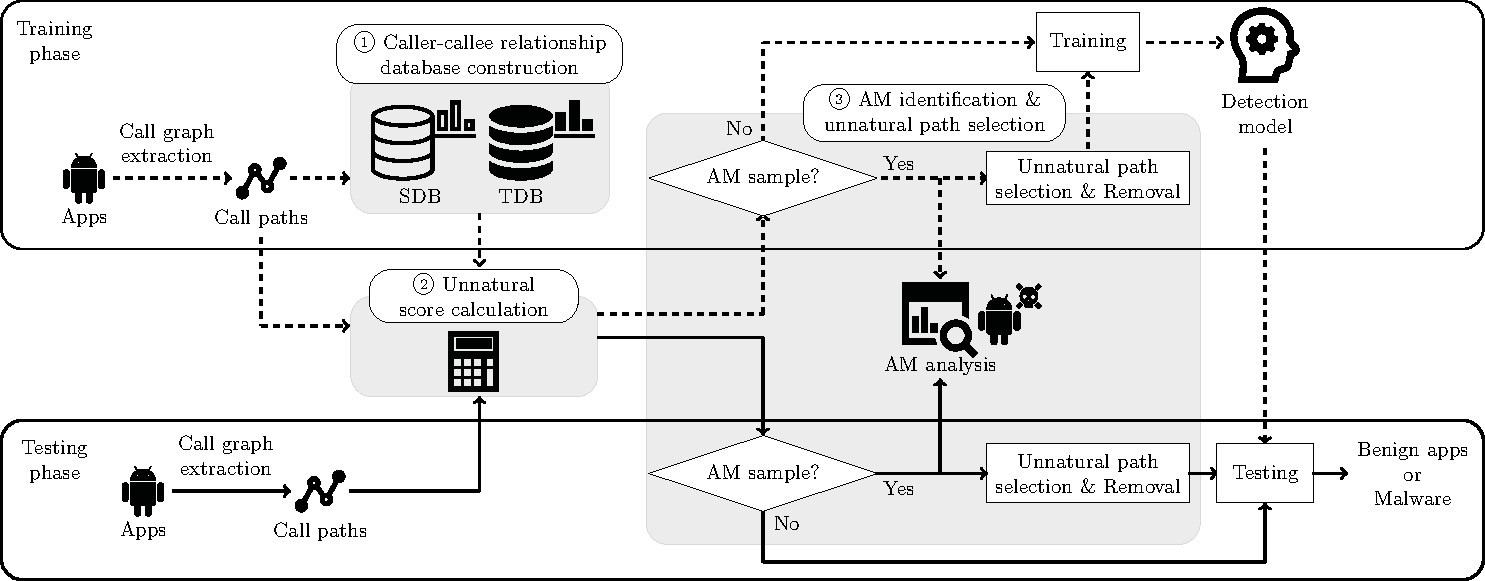
\includegraphics[scale=0.28]{./figures/overview.pdf}
 \caption{The overview of evasive techniques.} 
 \label{fig:ov}
\end{figure}
%\afterpage{\clearpage}

\subsubsection{Vulnerability against GSI manipulation}
The GSIs fed into the network as inputs in the previous scheme have pixels that match the Binary Data (BD), which is inserted into the source code by the compiler and has nothing to do with runtime behaviour \cite{am}.
Adversaries can make the CNN model cause false judge as benign by intentionally applying some noises to these pixel values \cite{am}.
The two GSIs shown in \figurename~\ref{fig:amGSI} are the actual GSIs of a malware before and after adding noise.
The noise is added to the GSI of AM by manipulating the pixel values of pixel that match metadata or debugging information which is irrelevant to the runtime behaviour.
By adding the noise in this way, the AM can mislead CNN as benign in the previous scheme.
The AM attack is a threat to CNN detection since it allows the classifier to intentionally judge the malware as benign while maintaining the original behaviour of malware.

\begin{figure}[h]
 \centering
 %\hspace{-55pt}
 \includegraphics[scale=0.28]{./figures/AM.pdf}
 \caption{The AM GSIs.} 
 \label{fig:amGSI}
\end{figure}
%\afterpage{\clearpage}
\subsubsection{Vulnerability against binary manipulation}
The binary which converts to a GSI can also be manipulated to evade the CNN detection by being obfuscated \cite{om}.
Due to the small computational resources, obfuscation techniques with packing tools, which also can compress the BD while encrypting, are tend to be used in IoT malware obfuscation field.
As shown in \figurename~\ref{fig:omGSI}, the original BD is compressed and encrypted at the same time, and new headers and tool-dependent data which do not contribute to the decision for detection are inserted.
In addition to the fact that malware obfuscated with the packing tools can be recovered and analyzed only at runtime, the encryption method differs depending on the packing tool.Thus, binary manipulation attack is a threat especially for IoT devices which are not suitable for dynamic analysis due to the limited computing resources since there is no way to statically analyze them in advance.

\begin{figure}[h]
 \centering
 %\hspace{-55pt}
 \includegraphics[scale=0.28]{./figures/OM.pdf}
 \caption{The OM GSIs.} 
 \label{fig:omGSI}
\end{figure}

\paragraph*{}
While previous scheme based on CNN can achieve high accuracy in detection, it is vulnerable against the above two attacks which aim to evade detection resulting in lower detection accuracy.
In fact, \tablename~\ref{tab:prev} shows the original accuracy and the degradation of them by each attack.
The accuracy, which achieves 99.8\%, drops to 66.1\% under the AM attack with GSI manipulation and 86.2\% under the OM attack with BD manipulation.
The results indicate that the previous scheme is vulnerable to these attacks.

Hence, in this reserch, I aim to propose defense methods against the evasive techniques on different targets, GSI and BD, for the practical use of static detection based on CNN.

\begin{table}[h]
  \begin{center}
    \caption{Detection accuracy of original/manipulated malware.}
    \label{tab:prev} 
    \begin{tabular}{|c|c|c|} \hline
       & Manipulation Target & Accuracy (\%) \\ \hline \hline
      Original Malware & no manipulation  & 99.8  \\ \hline
      AM & GSI & 66.1  \\ \hline 
      OM & BD & 86.2 \\ \hline
    \end{tabular}
  \end{center}
\end{table} 
%\afterpage{\clearpage}

\section{Proposed Scheme} \label{sec:proposed_scheme}
\subsection{Approach}
Our goal is to design the defense scheme against each evasive technique on different targets, GSI and BD, to achive the practical CNN based IoT malware detection on IoT devices.
In order to accomplish our goal, we propose an evasion-resilient IoT malware detection scheme with invalidating adversarial byte sequences and 1D convolutional filters.  
The main idea of our scheme is that there still remain regions which contribute to decision making in both manipulated targets after the attacks.
We aim to improve the detection accuracy by statically extracting/enhancing each valuable region of the target to the CNN model.

\figurename~\ref{fig:propAM} and \figurename~\ref{fig:propOM} show the manipulated area by adversaries and the area which have high degree of contribution for CNN to make decision on representative manipulated target.
The red area in each target is the area which has been manipulated.
In the case of AM, noise is added to the pixels, and in that of OM, the original BD is compressed or new code is inserted in these regions.
On the other hand, the yellow area is where contributes to decision making still remaining after the attack.
In the case of AM, it is the pixel region where noise cannot be added, and in that of OM, it is the byte sequence region which remain discretely after the compression.

In each defense scheme, the detection accuracy can be improved by feeding those yellow region effectively to the CNN model.
The representative schemes are explained in the following sections.

\begin{figure}[h]
 \centering
 \includegraphics[scale=0.28]{./figures/propAM.pdf}
 \caption{The valuable/manipulated regions in AM.} 
 \label{fig:propAM}
\end{figure}

\begin{figure}[h]
 \centering
 \includegraphics[scale=0.28]{./figures/propOM.pdf}
 \caption{The valuable/manipulated regions in OM.} 
 \label{fig:propOM}
\end{figure}
%\afterpage{\clearpage}
%\newpage

\subsection{Defense scheme against AM}
A defense scheme against AM, which is a malware whose GSI is manipulated, is explained in this section.

We focus on the fact that the adversary can manipulate only the pixels which match the BD whose information is unnecessary at runtime.
This is because the AM must maintain the original functionality of the malware even after the noise is added by the adversary.
In our proposal, we call these pixels Junk Pixels (JPs), and we think it would be possible to remove the noise by converting their pixel values into 0, which means turning them black pixels.

The two GSIs as shown in \figurename~\ref{fig:denoise} are the AM GSI with noise added by adversary and the that with denoising for JPs in our proposal.
The red box area is the area where the pixel values are converted into 0 as JPs.
This pixel region corresponds to the byte sequences which contain unnecessary information at runtime, such as metadata and debugging information used while linking.
Thus, they can be regarded as pixels where the noise which contribute to benign decision can be added when AMs are created.

On the other hand, yellow box area is the area with no manipulation in our proposal.
This pixel area corresponds to the byte sequences that represents the malware behaviour and the data held.
Thus, it is judged to hold valuable information for the classification since it is difficult to manipulate these byte sequences affecting the malware function for adversary without any destructions.
Hence, we utilize JPs, which locate in this area, for our detection as it is.

By doing this denoising process, the detection without being misled by AMs would be possible since only the pixels which tend to be not manipulated can be used for our classification.

\begin{figure}[h]
 \centering
 %\hspace{-55pt}
 \includegraphics[scale=0.28]{./figures/denoise.pdf}
 \caption{The difference with before and after denoising AM GSI.} 
 \label{fig:denoise}
\end{figure}
%\afterpage{\clearpage}
\subsection{Defense scheme against OM}
A defense scheme against OM, which is a malware whose BD is obfuscated with packing tools, is explained in this section.

In this defense scheme, we focus on the fact that the appearing order of discrete byte sequences remaining after obfuscation is invariant before and after packing.
Thus, showing the honrizontal connection of the byte sequences derived from the original BD can result in emphancizing valuable region remaining in OM for the CNN model.
We realize it by convoluting the GSI pixels in the horizontal direction with 1D filters.

I explain the method of convolution in the horizontal direction of pixels with a 1D Convolutional filter (1D Conv.), comparing with that in two dimentions with a 2D Convolutional filter (2D Conv.) filter in the previous scheme.
\figurename~\ref{fig:2d} shows the flow of the previous method using 2D convolutional filters, such as this blue flame, which are commonly used in image analysis due to correlation in both horizontal and vertical directions.
The figure with 6*6 squares in \figurename~\ref{fig:2d} represents the GSI, and each of them is a representaion of a pixel.
In particular, the yellow pixels represent pixels valuable information and the gray pixels represent pixels which are not necessary for classification due to tool-dependency.
Unlike common images, the correlation in the vertical direction is weak in GSIs since they are converted from byte sequences.
Furthermore, by convoluting with such 2D filters, both pixels, yellow ones and gray ones, coexist in the same filter especially in the convolution of the boundary of those pixel regions.
It can result in the false classification since the weight of valuable pixels in the decision becomes small in consequence of the useless pixels coexisting in the same filter.

On the other hand, in our proposal, the GSI is convoluted using 1D filters with a horizontal length as shown in the red frame in \figurename~\ref{fig:1d}, which represents the flow of the proposal method.
In our proposal, we can emphasize the byte regions which are valuable for classification by showing the correlation of the appearing order of discrete byte sequences remaining after obfuscation to the CNN model.
Furthermore, it is possible to avoid the degradation of valuable pixel weight by the pixel which has coexisted in the vertical direction in the previous method at the boundary of both pixels.

As described above, by using 1D filters to show the horizontal correlations between encrypted byte sequences, we can improve the detection accuracy by highlighting features retained in the OM which are valuable for training CNN model even under the static analysis.

\begin{figure}[h]
 \centering
 %\hspace{-55pt}
 \includegraphics[scale=0.28]{./figures/2d.pdf}
 \caption{The flow of convolution with 2D Conv..} 
 \label{fig:2d}
\end{figure}
\begin{figure}[h]
 \centering
 %\hspace{-55pt}
 \includegraphics[scale=0.26]{./figures/1d.pdf}
 \caption{The flow of convolution with 1D Conv..} 
 \label{fig:1d}
\end{figure}

\section{Evaluation} \label{sec:evaluation}
In order to demonstrate the effectiveness of our scheme, we evaluate Accuracy of each defense method compared to the previous scheme.
Accuracy is calculated as:
\begin{equation}
  \mathrm{Accuracy} = \frac{\mathrm{TP}+\mathrm{TN}}{\mathrm{TP} + \mathrm{TN} + \mathrm{FP} + \mathrm{FN}}, 
\end{equation}
where TP, TN, FP, and FN denote the number of True Positive (malware are regarded as malware), True Negative (benign files are regarded as benign ones), False Positive (benign files are regarded as malware), and False Negative (malware are regarded as benign files), respectively.  

\subsection{Simulaion parameters}
\begin{table}[h]
	\begin{center}
		\caption{Simulation Parameters.}
		\label{tab:simulation_parameters} 
		\begin{tabular}{|c|c|} \hline
			The name of parameters & Value\\ \hline \hline
			Benign files & Ubuntu 16.04.3\cite{ubuntu}\\ \hline
			\multirow{2}{*}{\hfill Malwares  \hfill} & IoTPOT\cite{iotpot} \\ 
																							 & VirusTotal\cite{virustotal}\\ \hline
			Number of benign files  & 1,442 \\  \hline
			Number of malware  &  7,263 \\ \hline
			AM attack method & White-box \cite{am, yamafumi} \\ \hline
			\multirow{2}{*}{\hfill Packing tools for OM  \hfill} & UPX\cite{upx} \\ & kiteshield\cite{kiteshield} \\ \hline
			Number of samples  & \multirow{2}{*}{\hfill 800 \hfill} \\  
			in AM-resiliency evaluation & \\ \hline 
			Number of samples  & \multirow{2}{*}{\hfill 1000 \hfill} \\  
			in OM-resiliency evaluation & \\ \hline 
		\end{tabular}
	\end{center}
\end{table} 

\tablename~\ref{tab:simulation_parameters} shows our simulation parameters.  

We use the benign files from Ubuntu system files \cite{ubuntu} as the begin files.
Meanwhile, malware are collected from IoTPOT \cite{iotpot} and VirusTotal \cite{virustotal} which is a repository of malware samples for security researchers.
In order to use those samples as inputs for CNN, we convert each sample to the correponding GSI by following the same procedures implemented in \cite{previous}.
In particular, a binary can be reformatted to a sequence whose elements are 8-bit strings.
Then, each string can be converted to a decimal number which can be seen as the value of a one-channel pixel.
After that, we rescale the GSIs to the size of 64*64 such that they can be input to the CNN.
In particular, manipulated malware for each attack are created with an adversarial technique implemented in \cite{am, yamafumi} and two packing tools \cite{upx, kiteshield} shown in \tablename~\ref{tab:simulation_parameters}.

In the case of AM-resiliency evaluation, we apply a white-box method as a adversarial technique for AM, where an the adversary knows the training data and the structure of the CNN model since it is currently the mainstream in this reserch field.

In the case of OM-resiliency evaluation, we use two packing tools, called UPX \cite{upx} and kiteshield \cite{kiteshield}, in order for malware to be obfuscated.
The UPX is a tool which is often utilized mainly for software compression purposes and, according to \cite{pack_research}, the use of it is confirmed in more than 50\% of obfuscated malware. 
Meanwhile, the kiteshield is a tool which is often utilized mainly for the purpose of encrypting softwares.
Especially, in this evaluation, we prepare three dataset on the basis of which tools to be used for their obfuscation in order to show the versatility in that our scheme is independent of the packing tools.
Two datasets of the three are composed of malware obfuscated by each packing tooks, UPX and kiteshield, and the other are mixed malware from those datasets. 

In the evaluation in respective evaluation, some of the samples from total manipulated malware, 800 samples in AM attack scenario and 1000 samples in OM attack scenario, are picked randomly, then utilized as inputs in order to keep balance between the number of malware and that of benign ones.

\subsection{Evaluation of the invalidating adversarial byte sequences against AM attack}
The effectiveness of the proposed method against AM which invalidates adversarial byte sequences with noise removal in the non-valuable pixels is shown in this subsection.
We compare the accuracy of our proposed scheme with that of the previous scheme as shown in \figurename~\ref{fig:evalAM}.
The left graph represents the accuracy of the previous scheme in detecting original malware, the middle one does that in detecting AM, and the right one does the accuracy of the proposal, where non-valuable pixel values in benign and AM samples are converted to zero.
As shown in \figurename~\ref{fig:evalAM}, the proposed scheme achieves improving the accuracy degraded by AM from 66.1\% to 99.4\%.
Although a slight decrease in detection accuracy is observed compared to the previous scheme and the proposal, the proposal is able to maintain high accuracy.
Thus, the loss of valuable information for classification by removing noise can be considered to be small.
Hence, we conclude that the proposed method against AM, where the non-valuable pixels at runtime are focused on, achieves a robust defense method which can invalidate adversarial techniques in AM.

\begin{figure}[h]
 \centering
 %\hspace{-100pt}
 \includegraphics[scale=0.35]{./figures/evalAM.pdf}
 \caption{The accuracy of the proposal aginst AM.} 
 \label{fig:evalAM}
\end{figure}
%\afterpage{\clearpage}

\subsection{Evaluation of the method with 1D convolutional filters against OM attack}
The effectiveness of the proposed method with 1D convolutional filters against OM is shown in this subsection.
We compare the accuracy of our proposed scheme using 1D Conv. with that of the previous scheme using 2D Conv. in each dataset as shown in \tablename~\ref{tab:evalOM}.
Compared to 2D Conv. in the previous scheme, the detection accuracy is improved by 1D Conv. in the proposal for all cases.
In the datasets where the both-tools-made OM are mixed in particular, the accuracy improves from 86.2\% to 90.0\%.
According to the result above, we conclude that the proposed method with 1D Conv. against OM achieves a robust defense method with less tool-dependency against OM.
\begin{table}[h]
  \begin{center}
    %\vspace{-8pt} 
    \caption{The datasets used for the OM-resiliency evaluation.}
    \label{tab:evalOM} 
    % \vspace{-8pt} 
    % \hspace{-10pt} 
    \begin{tabular}{|c|c|c|} \hline
      \multirow{2}{*}{\hfill  \hfill} & \multicolumn{2}{c|}{Accuracy}  \\ \cline{2-3} 
					     & Prev. (2D filters) & Prop. (1D filters) \\ \hline \hline
      UPX & 94.8\% & 96.2\% \\ \cline{1-3} 
      kiteshield & 85.0\% & 87.8\% \\ \cline{1-3} 
      mix & 86.2\% & 90.0\% \\ \cline{1-3} 
  \end{tabular}
  \end{center}
\end{table}

\paragraph{}
In order to observe the relation between the detection accuracy and the filter size of 1D Conv., we evaluate the accuracy varing the filter width.
The 1D Conv. size is changes based on the area of the 2D Conv., which is defined as $S$ in the evaluation, in the previous scheme.
The result is shown in \figurename~\ref{fig:evalOM}, where the red line indicates the accuracy of the proposed scheme and the blue one does that of the previous scheme.
In the range of $1/4S$ to $1.5S$, the accuracy increases as the filter size also increases, and reaches 90.0\% at $1.5S$.
The result suggests that a certain width is necessary to emphasize the appearing order to the CNN model, since the remaining original byte sequences is highly disjoint due to resizing during GSI conversion and compression by obfuscation procedures.
Meanwhile, the accuracy decreases from $1.5S$ to $2.0S$.
We consider that this is caused by the decrease in learning efficiency due to the increase in parameters caused by the expansion of the filter size.

\begin{figure}[h]
 \centering
 %\hspace{-100pt}
 \includegraphics[scale=0.35]{./figures/evalOM.pdf}
 \caption{The relation between the accuracy and 1D Conv. size of the proposal aginst OM.} 
 \label{fig:evalOM}
\end{figure}

\section{Limitation} \label{sec:limitation}
\section{Conclusion and future work} \label{sec:conclusion}
In this thesis, we have proposed an evasion-resilient IoT ,malware detection scheme with invalidating adversarial byte sequences and 1D convolutional filters. 
We utilize remaining regions which contribute to decision making in both manipulated targets, GSI and BD, even after the attacks.
In order to emphasize the valuable regions in GSI, the defense method converting JP values to zero is proposed aginst AM attacks.
On the other hand, in order to emphasize the valuable regions in BD, the defense method showing the horizontal connection of appearing order of byte sequences with 1D Conv. is proposed aginst OM attacks.
The defense methods of our scheme are effective in both cases.
In the evaluation of the method against AM, it improves detection accuracy without the loss of valuable information.
In the evaluation of the method against OM, it improves detection accuracy independent of the packing tool.
Furthermore, I discover the horizontal connections in encrypted byte regions and the efficiency of 1D Conv..

\bibliographystyle{IEEEtran}% bib style
\bibliography{IEEE_ref}

\begin{IEEEbiography}[{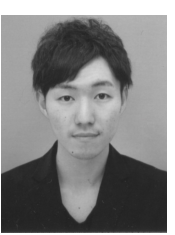
\includegraphics[width=1in,height=1.25in,clip,keepaspectratio]{./figures/kato.pdf}}]{Hiroya Kato} was born in Gunma, Japan in 1994. He received his B.E. and M.E. degrees from Keio University, in 2017 and 2019, respectively, where he is currently pursuing the Ph.D. degree. His research interest is security \& privacy for IoT. He is a member of IEICE.
\end{IEEEbiography} 

\begin{IEEEbiography}[{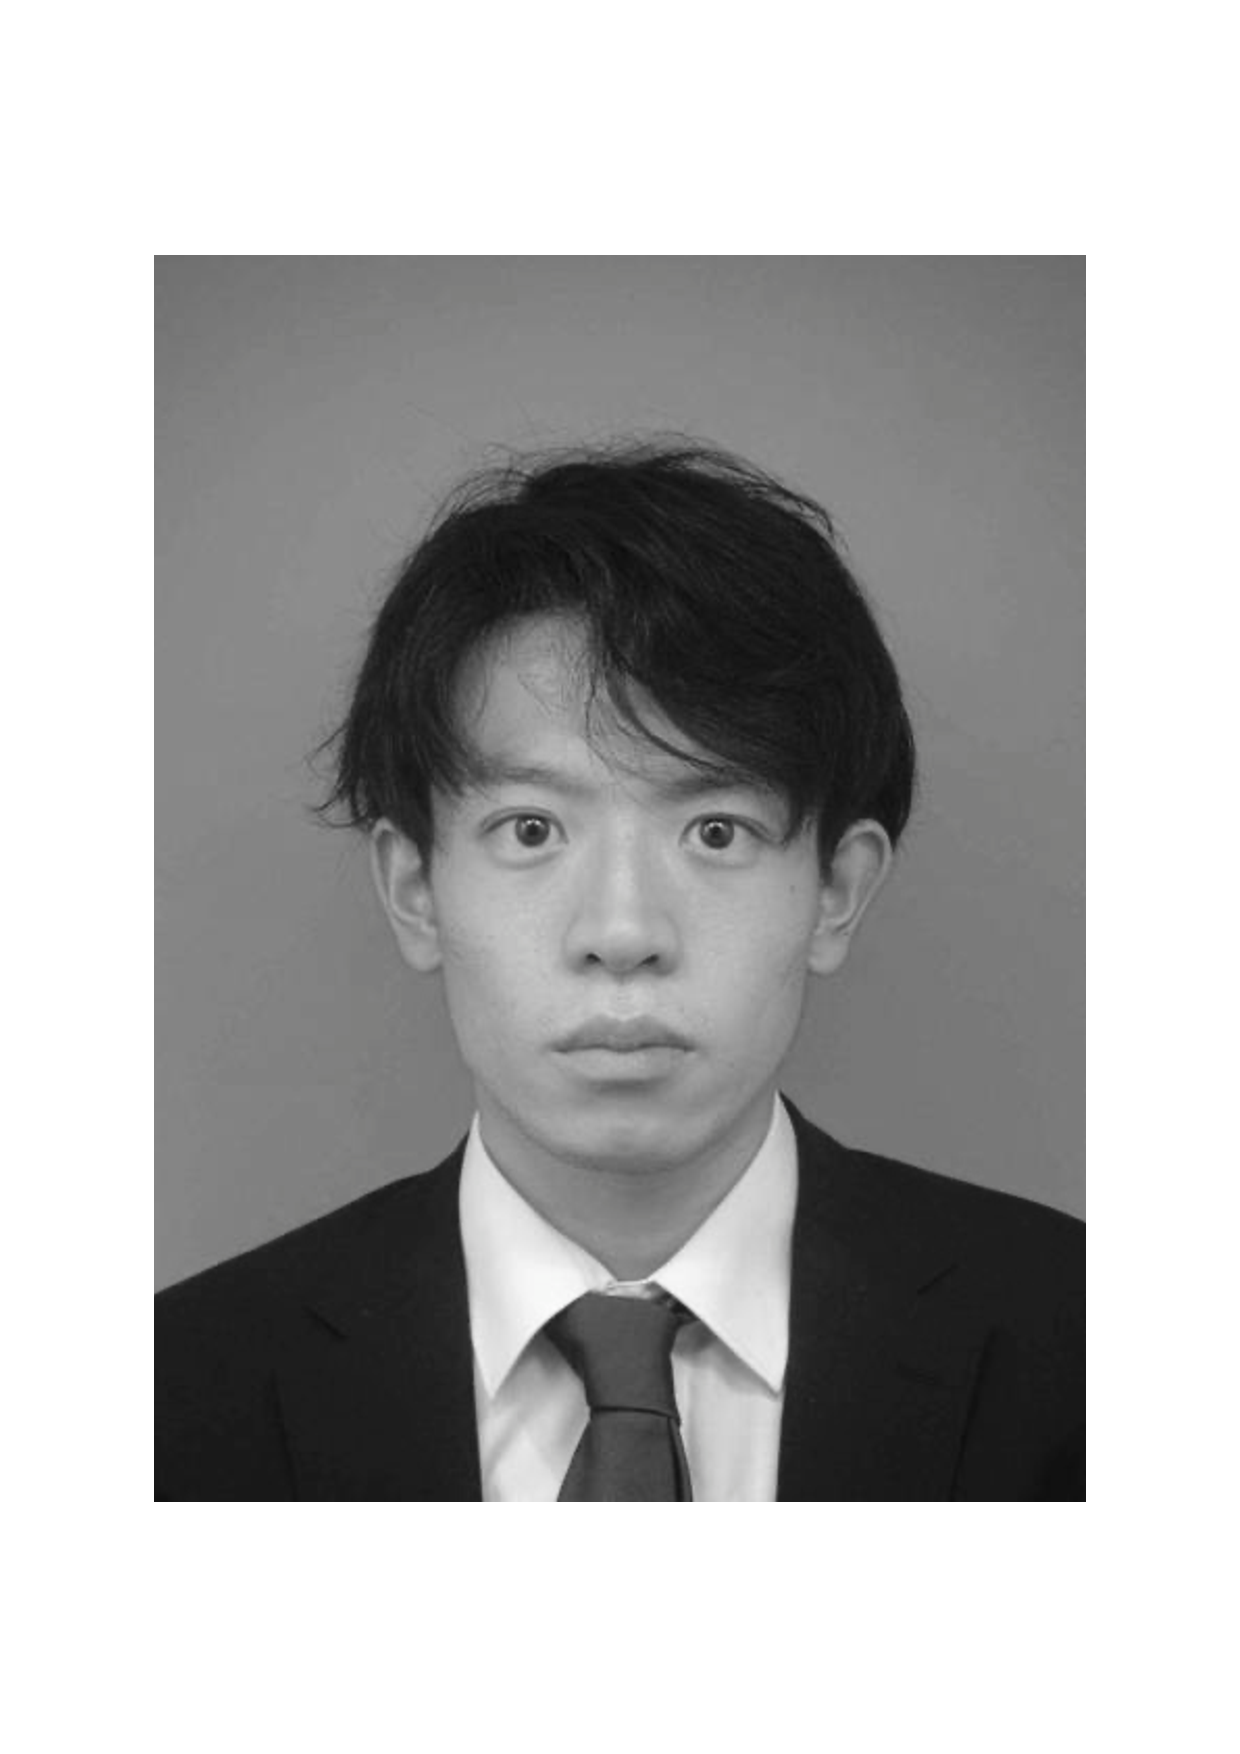
\includegraphics[width=1in,height=1.25in,clip,keepaspectratio]{./figures/sasak.pdf}}]{Takahiro Sasaki} was born in Saitama, Japan in 1995. He received his B.E. degrees from Keio University in 2021. His research interest is security \& privacy for IoT.
\end{IEEEbiography}

\begin{IEEEbiography}[{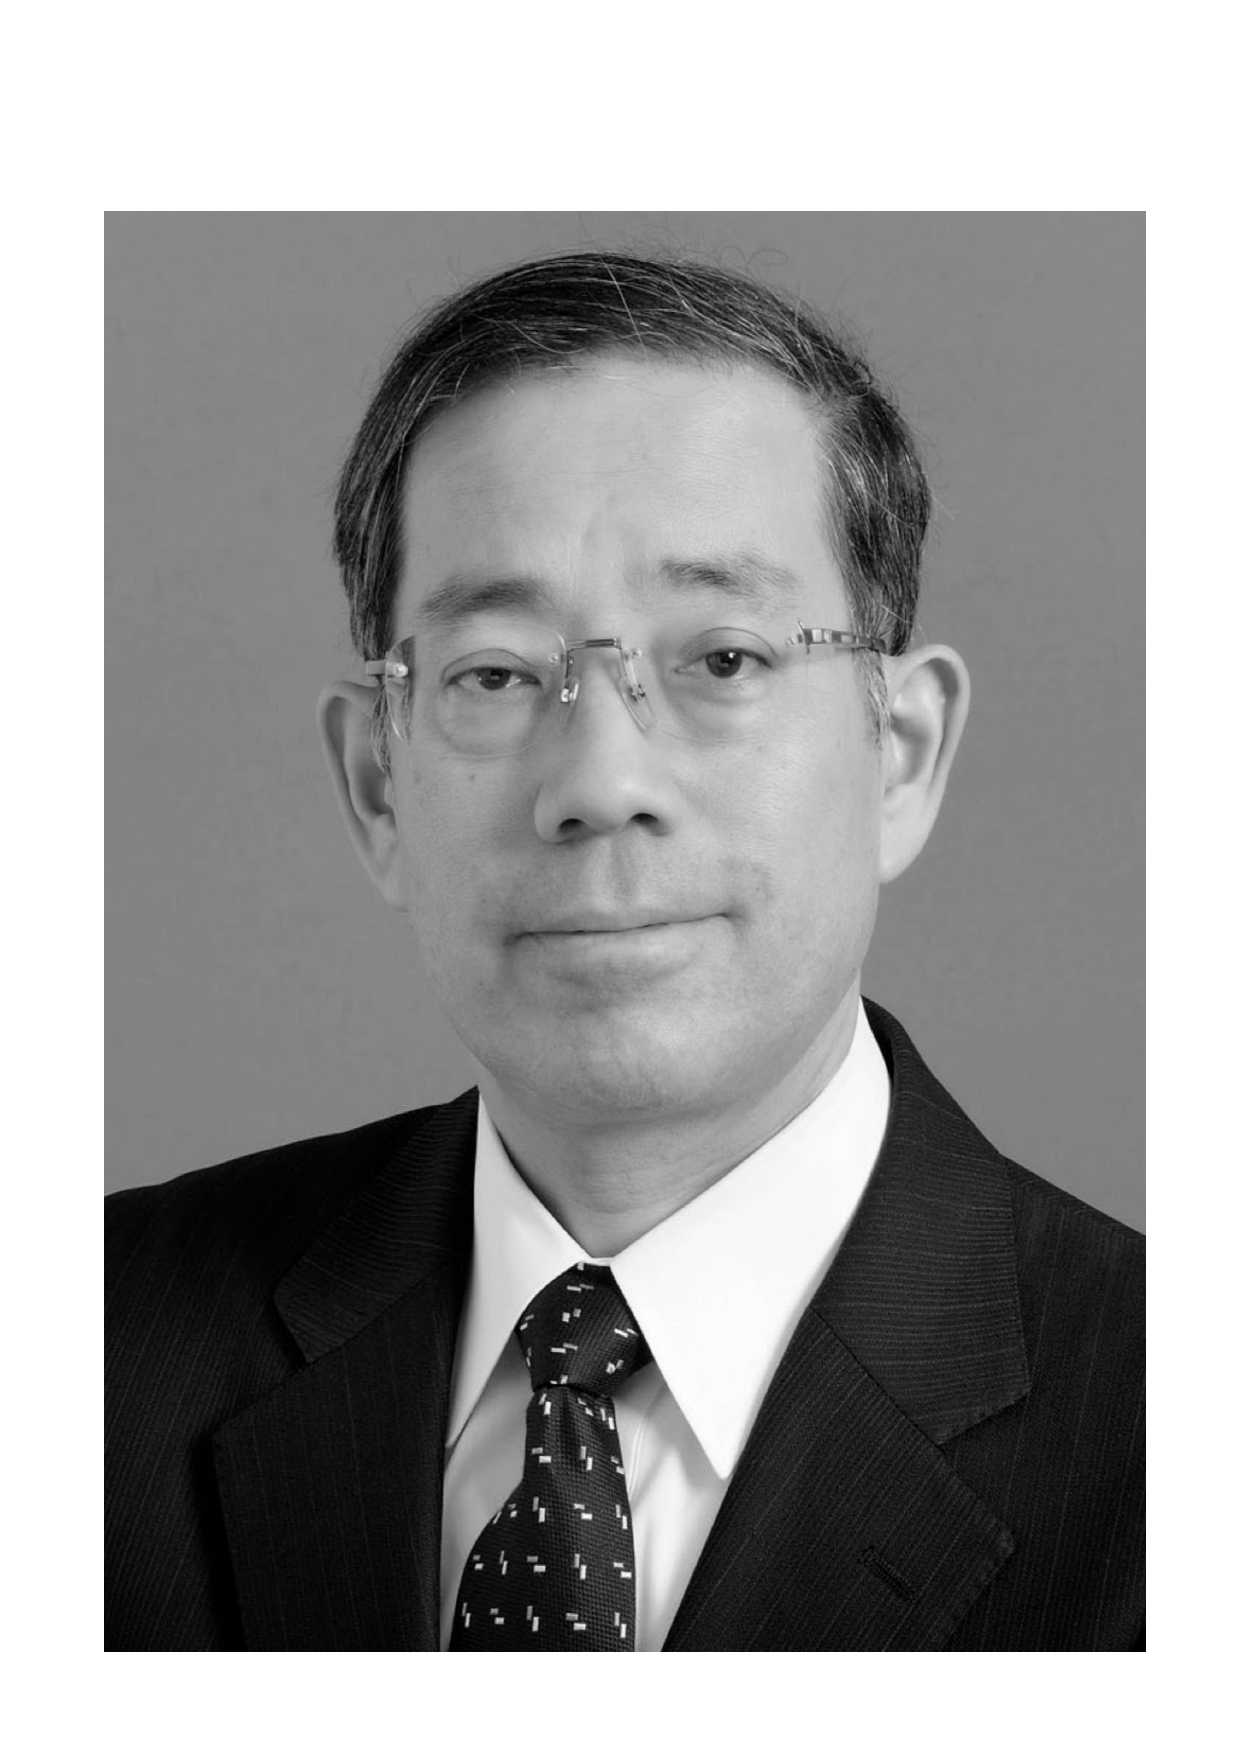
\includegraphics[width=1in,height=1.25in,clip,keepaspectratio]{./figures/sasas.pdf}}]{Iwao Sasase} was born in Osaka, Japan in 1956. He received the B.E., M.E., and D.Eng. degrees in Electrical Engineering from Keio University, Yokohama, Japan, in 1979, 1981 and 1984, respectively. From 1984 to 1986, he was a Post Doctoral Fellow and Lecturer of Electrical Engineering at the University of Ottawa,ON, Canada. He is currently a Professor of Information and Computer Science at Keio University, Yokohama, Japan. His research interests include modulation and coding, broadband mobile and  wireless communications, optical communications, communication networks and information theory. He has authored more than 301 journal papers and 446 international conference papers. He granted 48 Ph.D. degrees to his students in the above field. Dr. Sasase received the 1984 IEEE Communications Society (ComSoc) Student Paper Award (Region 10), 1986 Inoue Memorial Young Engineer Award, 1988 Hiroshi Ando Memorial Young EngineerAward, 1988 Shinohara MemorialYoung EngineerAward, 1996 Institute of Electronics, Information, and Communication Engineers (IEICE) of Japan Switching System Technical Group Best Paper Award, and WPMC2008 Best Paper Award. He is now serving as a Vice-President of IEICE. He served as President of the IEICE Communications Society (2012-2014). He was Board of Governors Member-at-Large (2010-2012), Japan Chapter Chair (2011-2012), Director of the Asia Pacific Region (2004-2005), Chair of the Satellite and Space Communications Technical Committee (2000-2002) of IEEE ComSoc., Vice President of the Communications Society (2004-2006), Chair of the Network System Technical Committee (2004-2006), Chair of the Communication System Technical Committee (2002-2004) of the IEICE Communications Society, Director of the Society of Information Theory and Its Applications in Japan (2001-2002). He is Fellow of IEICE, and Senior Member of IEEE, Member of the Information Processing Society of Japan.
\end{IEEEbiography}

\endgroup
\EOD
\end{document}
